%% And extended abstract addressing:
%% - Problem & motivation
%% - Background & related work
%% - Approach & uniqueness
%% - Results and contributions
%%
%% 2 pages, pdf. Reference lists don't count.
%% Options:
%% - acmart[sigplan]
%% - rntz, rntzgeometry[a5], pdfbook
%%   hm, need custom configuration...

\documentclass[sigplan,screen,dvipsnames]{acmart}
\settopmatter{printacmref=false}
\setcopyright{none}
\renewcommand\footnotetextcopyrightpermission[1]{}
\pagestyle{plain}

%\usepackage[scale=0.8]{librebaskerville}\linespread{.97}
\usepackage[scale=0.82]{librebaskerville}%\linespread{.995}

%\usepackage[scale=1.042]{cochineal}
%\usepackage[scale=0.94]{XCharter}\usepackage{eulervm}\edef\zeu@Scale{.972}



%% %% ---- Formatting ----
%% \documentclass[twocolumn,10pt]{extarticle}
%% \usepackage[dvipsnames]{xcolor}
%% \usepackage[a4,width=175mm]{rntzgeometry}
%% \setlength\columnsep{20pt}
%% \setlength\parskip{0pt}

%% %% TODO: smaller section titles
%% \usepackage{titlesec}    % (sub)section header styling
%% \titleformat*{\section}{\normalfont\large\bfseries}
%% \titleformat*{\subsection}{\normalfont\normalsize\bfseries}
%% \titlespacing{\section}{0pt}{.667em plus .1em minus .1em}{.3em plus .1em}

%% \usepackage[scale=1.0355]{cochineal}
%% \usepackage[semibold,scaled=.911]{sourcesanspro}
%% %\usepackage{biolinum}
%% \usepackage[scaled=.969]{inconsolata}
%% \usepackage[small]{eulervm}

%% \usepackage[spacing=true]{microtype}
%% \frenchspacing


%% ---- Packages ----
\usepackage{amsfonts,amsmath,latexsym,stmaryrd}
\usepackage{anyfontsize}
\usepackage{lipsum}
\usepackage{mathpartir}
\usepackage{mathtools}          % \dblcolon
\usepackage[nameinlink]{cleveref}
\usepackage{tikz,tikz-cd}
\usepackage{multirow}
\usepackage{booktabs}           % \midrule


%% ---- Commands ----
\newcommand\rulestyle{\sffamily}
\newcommand\rulename[1]{{\rulestyle#1}}

\newcommand\R{\mathbb{R}}
\newcommand\x\times
\newcommand\todo[1]{{\color{Purple}#1}}

\newcommand{\opcolor}{\color{ForestGreen}}
\newcommand{\isocolor}{\color{NavyBlue}}
\newcommand{\pathcolor}{\color{Bittersweet}}

\newcommand{\id}{\textrm{id}}
\newcommand{\op}{\textrm{\opcolor op}}
\newcommand{\iso}{{\texorpdfstring{\ensuremath{\isocolor\Box}}{iso}}}
\renewcommand{\path}{{\texorpdfstring{\ensuremath{\pathcolor\lozenge}}{path}}}

\newcommand{\idof}{\id\,}
\newcommand{\opof}{\op\,}
\newcommand{\isof}{\iso}
\newcommand{\pathof}{\path}

%% TODO: remove these.
\newcommand{\cid}{\id}
\newcommand{\cop}{{\opcolor\op}}
\newcommand{\ciso}{{\isocolor\iso}}
\newcommand{\cpath}{{\pathcolor\path}}

\newcommand\boxof{\kw{box}~}
\newcommand\h[3]{#1 : \left[#2\right] #3}
\newcommand\subtype[3]{\left[#1\right] #2 <: #3}

\newcommand\checksto{~\mathbf{checks}~}
\newcommand\infersto{~\mathbf{infers}~}
\newcommand{\checks}[5]{\h{#1}{#2}{#3} \vdash #4 \checksto #5}
\newcommand{\infers}[5]{\h{#1}{#2}{#3} \vdash #4 \infersto #5}


%% ---- Top matter ----
%%
%% Should include:
%% - Student author's name & email
%% - Institutional affiliation
%% - Research advisor's name
%% - ACM student member number
%% - Category (graduate or undergraduate)
%% - Research title
\title{Type inference for monotonicity}
\author{Michael Arntzenius, a PhD student ...}
\email{daekharel@gmail.com}
\affiliation{University of Birmingham}

% arg, should this be Neel or Dan? Neel, probably.
\author{... advised by Neelakantan R. Krishnaswami}
\email{neelakantan.krishnaswami@gmail.com}
\affiliation{University of Cambridge}


\begin{document}

\maketitle


\section{Problem \& motivation}
%% Clearly state the problem being addressed and explain the reasons for seeking
%% a solution to this problem.

Quick: which of these are monotone in $x$?\footnote{Whenever I say ``monotone''
  I mean ``monotonically nondecreasing'': $f$ is monotone iff $x \le y \implies
  f(x) \le f(y)$.}
%
\begin{mathpar}
  x - \log x

  x + 2^x

  {-2}x

  4
\end{mathpar}

Now, how did you \emph{know}?
%
Did you prove that $x \le y$ implies
%$x + \log x \le y + \log y$?
$x + 2^x \le y + 2^y$?
%
I didn't. I used a shortcut: compositional reasoning. Addition is monotone, and
so is $2^x$; so $x + 2^x$ must be as well.
%
And when I hear ``compositional reasoning'', I think ``type system''.

I aim to give a type system that can statically guarantee a function is monotone.
%
%Moreover, I aim to be able to \emph{infer} whether functions are monotone in their arguments without requiring any annotations other than type annotations.
%
This system is flexible---capable, for example, of typing a function $f : A \x
B \to C$ which is monotone in $A$ but not $B$.
%
It handles several flavors (or \emph{modes}) of function: ordinary (or
\emph{invariant}), monotone, antitone, and bivariant (both mono- and anti-tone).
%
And it requires no changes to terms besides type annotations.

What use might a type system guaranteeing monotonicity of certain functions be?
%
Well, monotonicity

\todo{
\begin{itemize}
\item Monotonicity for fixed points in Datafun
\item Monotonicity for eventual consistency
\item LVars????
\end{itemize}
}

%{\color{MidnightBlue}\lipsum[4]}


\section{Background \& related work}

\todo{
Describe the specialized (but pertinent) background necessary to appreciate
the work in the context of ICFP areas of interest. Include references to the
literature where appropriate, and briefly explain where your work departs
from that done by others.
}

\newcommand\mto{\overset{+}{\to}}

I extend prior work on Datafun~\citep{datafun}, a pure, total functional
language inspired by the deductive database language Datalog~\citep{datalog}.
%
Like Datalog, Datafun allows recursive queries, computed by iteration to a fixed point. To ensure termination, the iterated function must be monotone.
%
Datafun's original type system has \emph{two separate} function types, ordinary
and monotone; it cannot type a function $A \x B \to C$ monotone in $A$ but not
$B$. I aim to remove this restriction. Besides monotonicity, understanding
Datafun's features is not necessary for the present work.

I use bidirectional type inference \cite{bidirectional} to check programs' types. This requires some type annotations, but is simpler to describe and implement than full Damas-Milner inference. \todo{Explain how bidirectional inference works by splitting things into inferring \& checking forms, briefly.} Extending the scheme presented here to full type inference is left to future work.

%% Problems with Datafun as published:
%% - can't have f : A * B -> C monotone in A but not B
%% - doesn't handle antitone functions

\todo{TODO: Pfenning-Davies, Monotonicity Types, variance analysis?, that static analysis someone's pointed out}


\section{Approach \& uniqueness}
\todo{Describe your approach in addressing the problem and clear\-ly state how
  your approach is novel.}

%% - interpret everything in Preorder
%%
%% - infer how variables are used, entirely bottom-up (novel!)
%%
%% - use modal subtyping to handle mismatches between inferred & expected types, and to handle function application (novel!)
%%
%% - use distribution of modes to handle pattern-matching (novel?)

%% novel: modes for monotonicity! (not special kinds of functions, as in Datafun & Monotonicity Types)
%%
%% novel: higher-order! unlike Monotonicity Types!
%%
%% no intro/elim annotations! unlike Pfenning-Davies, certainly, or basically any modal approach?
%%
%% but how does it differ from variance typing?

\begin{center}
  \begin{tabular}{clc@{\hskip 0.25em}c@{\hskip 0.25em}ll}
    {\textit{Tone}}
    & {\textit{Name}}
    & \multicolumn{3}{c}{\textit{Transformation on $A$}}
    \\\midrule
    \cid & monotone
    & $a \le b : A$ &$\iff$& $a \le b : \idof A$
    \\
    \cop & antitone
    & $a \ge b : A$ &$\iff$& $a \le b : \opof A$
    \\
    \ciso & invariant
    & $a \le b \wedge b \le a : A$ &$\iff$& $a \le b : \isof A$
    \\
    \cpath{} & bivariant
    & $a \le b \vee b \le a : A$ &$\ \implies$& $a \le b : \pathof A$
    %% & {\small\itshape see \ref{sec:defining-path}}
  \end{tabular}
\end{center}


\subsection{Inferring usage bottom-up}

\todo{TODO explain pair rule}
\[\infer[\rulestyle pair]{
  \checks{x}{T}{A}{e_1}{B_1} \\
  \checks{x}{U}{A}{e_2}{B_2}
}{
  \checks{x}{T\wedge U}{A}{(e_1,e_2)}{B_1 \x B_2}
}
\]

\newcommand{\kw}[1]{\textrm{#1}}
\newcommand{\elet}[1]{\kw{let}~#1~\kw{in}~}

\todo{TODO explain let-binding rule}
\[\infer[\rulestyle let]{
  \infers{x}{T}{A}{e_1}{B} \\
  \checks{y}{U}{B}{e_2}{C}
}{
  \checks{x}{UT}{A}{\elet{y = e_1} e_2}{C}
}
\]

\begin{figure}
  \begin{mathpar}
    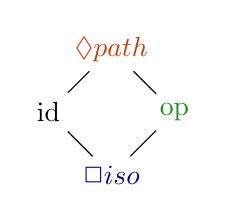
\begin{tikzpicture}[scale=0.8,baseline=(current bounding box.center)]
      \node (top)  at ( 0, 1) {$\cpath$};
      \node (bot)  at ( 0,-1) {$\ciso$};
      \node (-1)   at (-1, 0) {$\cid$};
      \node (1)    at ( 1, 0) {$\cop$};
      \draw (top) -- (-1) -- (bot) -- (1) -- (top);
    \end{tikzpicture}
    %%
    %% \begin{array}{r|cccc}
    %%   T \wedge U
    %%   & \cid & \cpath & \cop & \ciso\\\hline
    %%   \cid & \cid & \cid & \ciso & \ciso\\
    %%   \cpath & \cid & \cpath & \cop & \ciso\\
    %%   \cop & \ciso & \cop & \cop & \ciso\\
    %%   \ciso & \ciso & \ciso & \ciso & \ciso
    %% \end{array}

    \begin{array}{cr|cccc}
      \multicolumn{2}{c|}{\multirow{2}{*}{$UT$}}
      & \multicolumn{4}{c}{T}\\
      && \cid & \cop & \ciso & \cpath\\\hline
      \multirow{4}{*}{$U$}
      & \cid & \cid & \cop & \ciso & \cpath\\
      & \cop & \cop & \cid & \ciso & \cpath\\
      & \ciso & \ciso & \ciso & \ciso & \cpath\\
      & \cpath & \cpath & \cpath & \ciso & \cpath
    \end{array}
  \end{mathpar}

  \caption{Tone lattice and composition}
  \label{fig:tone-ops}
\end{figure}

\subsection{Modal subtyping}


\section{Results and contributions}
\todo{Clearly show how the results of your work contribute to programming
  language design and implementation in particular and to computer science in
  general; explain the significance of those results.}

% Makes Datafun more flexible.
% - functions f : A * B -> C
% - handles antitonicity for e.g. parity-stratified negation
% - no need to annotate case-expressions

% Suggests a novel approach to modal type systems that could, in some circumstances, result in fewer annotations and more ``natural'' code.


%% Bibliography
\bibliographystyle{abbrvnat}
\bibliography{datafun}

\end{document}
